%\documentclass[handout]{ximera}
\documentclass[nooutcomes]{ximera}

\usepackage{gensymb}
\usepackage{tabularx}
\usepackage{mdframed}
\usepackage{pdfpages}
%\usepackage{chngcntr}

\let\problem\relax
\let\endproblem\relax

\newcommand{\property}[2]{#1#2}




\newtheoremstyle{SlantTheorem}{\topsep}{\fill}%%% space between body and thm
 {\slshape}                      %%% Thm body font
 {}                              %%% Indent amount (empty = no indent)
 {\bfseries\sffamily}            %%% Thm head font
 {}                              %%% Punctuation after thm head
 {3ex}                           %%% Space after thm head
 {\thmname{#1}\thmnumber{ #2}\thmnote{ \bfseries(#3)}} %%% Thm head spec
\theoremstyle{SlantTheorem}
\newtheorem{problem}{Problem}[]

%\counterwithin*{problem}{section}



%%%%%%%%%%%%%%%%%%%%%%%%%%%%Jenny's code%%%%%%%%%%%%%%%%%%%%

%%% Solution environment
%\newenvironment{solution}{
%\ifhandout\setbox0\vbox\bgroup\else
%\begin{trivlist}\item[\hskip \labelsep\small\itshape\bfseries Solution\hspace{2ex}]
%\par\noindent\upshape\small
%\fi}
%{\ifhandout\egroup\else
%\end{trivlist}
%\fi}
%
%
%%% instructorIntro environment
%\ifhandout
%\newenvironment{instructorIntro}[1][false]%
%{%
%\def\givenatend{\boolean{#1}}\ifthenelse{\boolean{#1}}{\begin{trivlist}\item}{\setbox0\vbox\bgroup}{}
%}
%{%
%\ifthenelse{\givenatend}{\end{trivlist}}{\egroup}{}
%}
%\else
%\newenvironment{instructorIntro}[1][false]%
%{%
%  \ifthenelse{\boolean{#1}}{\begin{trivlist}\item[\hskip \labelsep\bfseries Instructor Notes:\hspace{2ex}]}
%{\begin{trivlist}\item[\hskip \labelsep\bfseries Instructor Notes:\hspace{2ex}]}
%{}
%}
%% %% line at the bottom} 
%{\end{trivlist}\par\addvspace{.5ex}\nobreak\noindent\hung} 
%\fi
%
%


\let\instructorNotes\relax
\let\endinstructorNotes\relax
%%% instructorNotes environment
\ifhandout
\newenvironment{instructorNotes}[1][false]%
{%
\def\givenatend{\boolean{#1}}\ifthenelse{\boolean{#1}}{\begin{trivlist}\item}{\setbox0\vbox\bgroup}{}
}
{%
\ifthenelse{\givenatend}{\end{trivlist}}{\egroup}{}
}
\else
\newenvironment{instructorNotes}[1][false]%
{%
  \ifthenelse{\boolean{#1}}{\begin{trivlist}\item[\hskip \labelsep\bfseries {\Large Instructor Notes: \\} \hspace{\textwidth} ]}
{\begin{trivlist}\item[\hskip \labelsep\bfseries {\Large Instructor Notes: \\} \hspace{\textwidth} ]}
{}
}
{\end{trivlist}}
\fi


%% Suggested Timing
\newcommand{\timing}[1]{{\bf Suggested Timing: \hspace{2ex}} #1}




\hypersetup{
    colorlinks=true,       % false: boxed links; true: colored links
    linkcolor=blue,          % color of internal links (change box color with linkbordercolor)
    citecolor=green,        % color of links to bibliography
    filecolor=magenta,      % color of file links
    urlcolor=cyan           % color of external links
}

\title{Rep-Tiles}
\author{Bart Snapp and Brad Findell}

\outcome{Learning outcome goes here.}

\begin{document}
\begin{abstract}
  We study self-similar shapes called rep-tiles.
\end{abstract}
\maketitle

\begin{teachingnote}
Problems 1--3 can be a preactivity.  

Supplies: scissors, printed versions of the figures (so that students can cut them out), and a printed version of the summary table.   Students will need some time working with the figures, computing their areas and perimeters, and practicing arithmetic of radicals.   

An overall goal (across these activities and related homework) is that students use dimension to think about scaling. This needs development and discussion.  
\end{teachingnote}

A \textbf{rep-tile}\index{rep-tile} is a polygon where several copies of
a given rep-tile fit together to make a larger, similar, version of
itself. If $2$ copies are used, we call it a \textit{rep-2-tile}, if
$3$ copies are used, we call it a \textit{rep-3-tile}, and if $n$ copies
are used, we call it a \textit{rep-n-tile}.  Below is an example of a rectangle 
that is a rep-4-tile.
\begin{image}
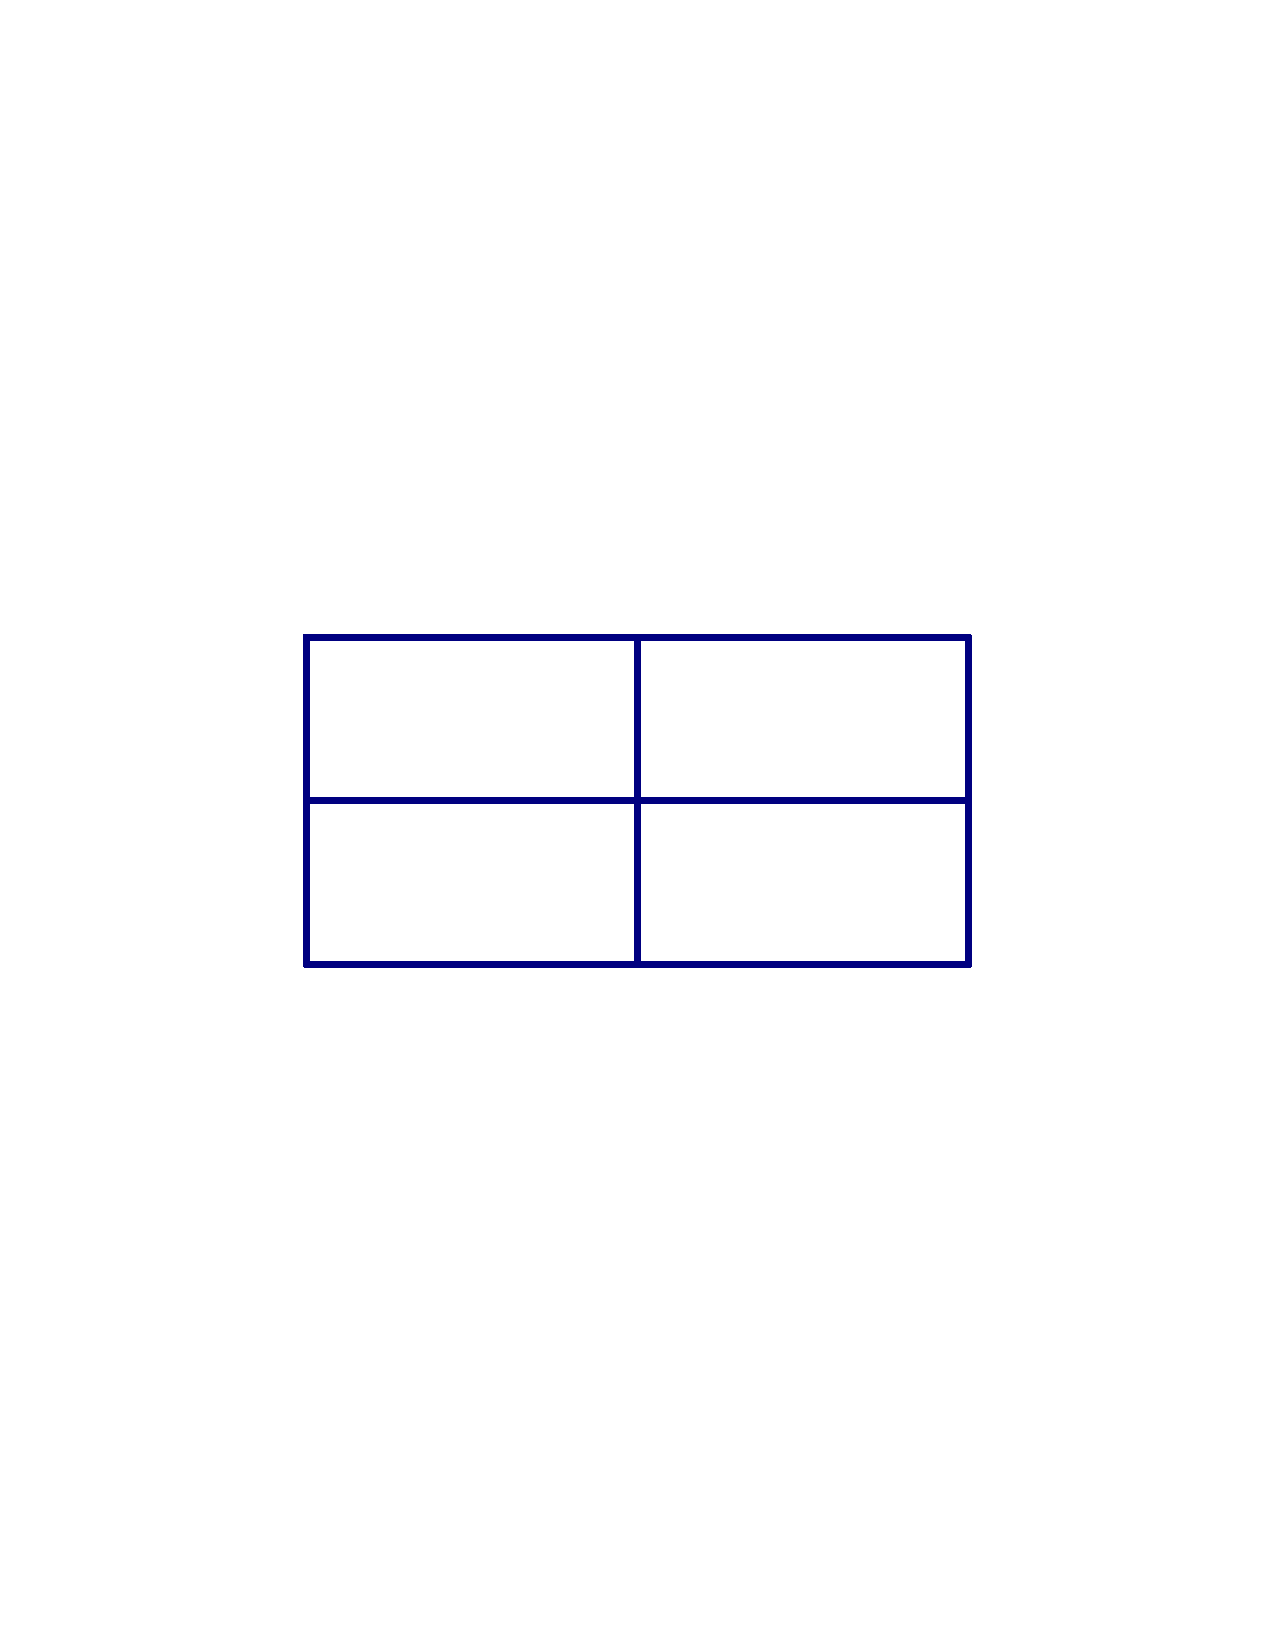
\includegraphics[scale=0.6]{reptile1.pdf}
\end{image}
\begin{problem}
Explain why every parallelogram is a rep-4-tile. Give an example, and compare the perimeter and area of the larger figure to that of the original.
\end{problem}

\begin{problem}
Explain why every triangle is a rep-4-tile. Give an example, and compare the perimeter and area of the larger figure to that of the
original.
\end{problem}

\begin{problem}
Explain why every parallelogram and every triangle is a rep-9-tile. Give an example of each, and compare the perimeter and area of the larger triangle to that of the original. Can you generalize your result?  In other words, for what values of $n$ can you say that every parallelogram and every triangle is a rep-$n$-tile?  
\end{problem}

\begin{problem}
With a separate sheet of paper, draw and cut out:
\begin{enumerate}
\item An isosceles right triangle whose sides have lengths $1''$, $1''$, and $\sqrt{2}''$.
\item A rectangle whose sides have lengths $1''$ and $\sqrt{2}''$.
\end{enumerate}
Working with a partner, show that each of these polygons is a rep-2-tile.  And in each case,
how do the perimeter and area of the larger polygon compare to the perimeter and area of the original?
\end{problem}

\begin{problem}
With a fresh sheet of paper, start a table to summarize your work so far.  Use \textbf{exact} answers whenever possible.
\begin{center}
\begin{tabular}{c|c|c|c}
rep-tile & scale factor (new:old) &  perimeter (new:old) &  area (new:old)  \\ \hline\hline
\textit{description} &     &      &     \\ 
  $\vdots$    & $\vdots$  &  $\vdots$  &  $\vdots$ \\ 
\end{tabular}
\end{center}
\end{problem}


\begin{problem}
Geometry Giorgio suggests that a rectangle whose sides have lengths
$1''$ and $4''$ is also a rep-2-tile. Is he right? If you should
happen to search the Internet for other examples of rep-2-tiles, you
might find a surprise.
\end{problem}


\begin{problem}
With a separate sheet of paper, draw and cut-out:
\begin{enumerate}
\item A 30-60-90 right triangle whose shortest side has length $1''$.
\item A rectangle whose sides have lengths $1''$ and $\sqrt{3}''$.
\end{enumerate}
Working with a partner, show that each of these polygons is a rep-3-tile.
\end{problem}

\begin{problem}
For each rep-tile above, compute the perimeter and area. In each case,
how does this relate to the perimeter and area of the larger polygon?
Add this information to your table.
\end{problem}

\end{document}
